%%%%% ------------------------------------------------------------------------------------------
%%
%%                               Document Template
%%
%%  Project Name: njustThesis
%%  Repository: https://github.com/jiec827/njustThesis
%%
%%%%% ------------------------------------------------------------------------------------------
%% re-written by Jie Cheng <jie.cheng@aliyun.com>
%% Last-modified: 2015-01-05
%%
%% This program can be redistributed and/or modified under the terms
%% of the GNU Public License, version 2.
%%%%% ------------------------------------------------------------------------------------------
%%
%%%%*************************Document Class Declaration*******************************
%%
\documentclass[UTF-8,AutoFakeBold]{sty/njustThesis}% thesis template of the Nanjing Univ of Sci & Tech
%% Options:
%% [draftinfo] % show draft version information
%%%%% --------------------------------------------------------------------------------
%%
%%%%**************************Command Define and Settings***************************
%%
\usepackage[njust]{sty/commons}% common settings
\usepackage{fontspec}
\usepackage{sty/custom}% user defined commands
\usepackage{pifont}
\usepackage[perpage,symbol*]{footmisc}
\DefineFNsymbols{circled}{{\ding{192}}{\ding{193}}{\ding{194}}
	{\ding{195}}{\ding{196}}{\ding{197}}{\ding{198}}{\ding{199}}{\ding{200}}{\ding{201}}}
\setfnsymbol{circled}
%%%%% ------------------------------------------------------------------------------------------
%%%%*********************************Content**********************************************
%%
\begin{document}
%%
%%%%% ------------------------------------------------------------------------------------------
%%
%%%%*********************************Frontmatter******************************************
%%
%% Frontmatter of Title page, Table of contents, Preface chapter.
%%
%% >>> Cover
%%
\setmainfont{Times New Roman}
%%
%%% >>> Title Page
%%
%%
%%%%********************** Chinese Title Page **************************************** 
%%
  \classification{}
  \confidential{}
  \UDC{}
%% 标题格式 \title[short title for headers]{Long title of thesis}
  \title[南理工学位论文\LaTeX{}模板]{南京理工大学学位\\论文\LaTeX{}模板}
  \titleUpp{南京理工大学学位}
  \titleLow{论文\LaTeX{}模板}
  \author{xxx}
  \authorNumber{920xxxxxxxxx}
  \advisor{xxx}
  \advisortitle{教授}
  \coadvisor{XXX}
  \coadvisortitle{教授}
  \degree{xx学院}
  \major{xxxx}
  \interest{xx}
  \school{南\hspace{5pt} 京\hspace{5pt} 理\hspace{5pt} 工\hspace{5pt} 大\hspace{5pt} 学}
  \submitdate{2024.05}
  \incoverdate{2024年06月}
  %
  \titleBackbone{南\\京\\理\\工\\大\\学\\学\\位\\论\\文\\模\\板}
  \schoolBackbone{南\\京\\理\\工\\大\\学}
%%
%%%%********************** English Title Page **************************************** 
%%
  \englishtitle{Template for Degree Thesis in NJUST \\ (\LaTeX)}
  \englishauthor{xxxxxxx}
  \englishadvisor{xxx xxx}
    \englishcoadvisor{xxx xxx}
  \englishinstitute{Nanjing University of Science \& Technology}
  \englishdate{June, 2024}
  \englishdegree{Dissertation}
%%
%%%%********************** Generate CHN & Eng Title *********************************** 
%%% 
%%
\maketitle
%%
\makeincovertitle
%%
\makeenglishtitle
%% make statement page
\makeatletter
\cleardoublepage
\thispagestyle{empty}
\begin{center}
\statement{
本学位论文是我在导师的指导下取得的研究成果,尽我所知,在本 学位论文中,除了加以标注和致谢的部分外,不包含其他人已经发表或 公布过的研究成果,也不包含我为获得任何教育机构的学位或学历而使 用过的材料。与我一同工作的同事对本学位论文做出的贡献均已在论文 中作了明确的说明。
}%

\accredit{
南京理工大学有权保存本学位论文的电子和纸质文档,可以借阅或 上网公布本学位论文的部分或全部内容,可以向有关部门或机构送交并 授权其保存、借阅或上网公布本学位论文的部分或全部内容。对于保密 论文,按保密的有关规定和程序处理。
}%

\end{center}
\clearpage
\if@twoside
  \thispagestyle{empty}
  \cleardoublepage
\fi
 \makeatother
%%%%*********************************** END *******************************************

%%
%% >>> start frontmatter page No.
%%
\frontmatter
%%
%% >>> Abstract
%%
\begin{abstract}

本文是南京理工大学学位论文模板——njustThesis的使用说明文档。主要内容为介绍\LaTeX{}文档类njustThesis的用法,以及如何使用\LaTeX{}快速高效地撰写学位论文。

\LaTeX{}是一种基于\TeX{}的排版系统,主要利用命令行代码的形式对文稿进行格式化处理。相对于常用的可视化工具(如MS Word$^{\circledR}$)而言,其能够让作者更加专注于文章本身内容,而较多地将排版等重复任务交给编译系统,尤其是数学公式、参考文献或图标较多的科技文献。针对中文,\LaTeX{}提供有CTeX套装,并且国内较多院校都提供有\LaTeX{}格式的学位论文模板,中文期刊的排版系统中应用也较为广泛。

对于学位论文而言,\LaTeX{}又是体现在模块化处理、公式、图标、交叉引用等方面。模块化处理即将整个文稿切割成多个简单的子模块,然后利用主文件将文稿的子模块链接成一篇完整的文章(和编程语言中模块化、以及商业软件LsDYNA$^{\circledR}$中使用的include命令相同)。另外,排版系统中的格式定义系统也可以单独的模块化,由类文件(.cls)通过命令定义文中需要的版式等格式函数命令,通过格式文件(.sty)包含一些常用的包(package)。如此,文章中的格式信息和文稿中的内容就形成了相对独立的系统。对普通用户而言,只需要书写文稿内容,而将格式信息交由专业排版方进行(如图书馆、出版社等)。公式和图表的优势体现在,格式自动化对齐(相信使用MS的都有过公式窜行和表格窜页的感触)、交叉引用自动编号。

在模块化的基础上,本文模板将南京理工大学学位论文格式进行标准化处理,方便使用方快速查找需要添加的文稿位置。文件夹架构是标准化的基础,将格式信息、文本内容、插图、文献分别布置在sty、tex、img和bib四个文件夹下,由主模块myThesis.tex进行流程控制。

对于用户而言,使用步骤较为简单(注意:中文的文本编辑应采用UTF-8):

1. 下载模版包(https://github.com/jiec827/njustThesis),解压;

2. 修改学位论文信息(tex/cover.tex),并将对应的内容添加至tex目录下的其他文件内(正文部分额外添加的章节需要在myThesis.tex文件中使用input命令包含);

3. 采用命令{\color{blue}xelatex myThesis.tex}进行编译;

4. 命令行{\color{blue}makeindex myThesis.nlo -s nomencl.ist -o myThesis.nls}生成图表引用和术语链接;

5. 命令行{\color{blue}bibtex myThesis.aux}更新参考文献引用;

6. {\color{blue}xelatex myThesis.tex}重新编译生成pdf文件。

为了更好的完成学位论文这种长篇幅的文稿排版,对格式文件的了解也是有必要的。首先从主文件myThesis.tex着手,把握真个流程思路与文章的对应关系。然后看格式文件/sty,可以从njustThesis.cls开始,.cfg和.sty较为简单,只是包含一些需要使用的常量、默认值和扩展包等。

小提醒:学习的宝典当然还是google$^{\circledR}$和baidu$^{\circledR}$哦!

本文初衷是趁双旦闲暇,给以后的学位论文排版做点准备工作。有感于开源的精神,特把排版代码放到GitHub$^{\circledR}$上,在开发过程中虽然是以参考和借鉴为主,但仍按照Repository的软件工程开源流程进行操作。希望能够有人多多参与,通过这个简单的开源项目,了解、学习和推广。当然,回到根本,希望这个基于\LaTeX{}的排版项目能够给更多的同学提供一点小帮助。

\keywords{南京理工大学,学位论文,\LaTeX{},模板}
\end{abstract}


\begin{englishabstract}

1 In the beginning was the Word, and the Word was with God, and the Word was God. 2 He was with God in the beginning. 3 Through him all things were made; without him nothing was made that has been made. 4 In him was life, and that life was the light of all mankind. 5 The light shines in the darkness, and the darkness has not overcome it.

6 There was a man sent from God whose name was John. 7 He came as a witness to testify concerning that light, so that through him all might believe. 8 He himself was not the light; he came only as a witness to the light.

9 The true light that gives light to everyone was coming into the world. 10 He was in the world, and though the world was made through him, the world did not recognize him. 11 He came to that which was his own, but his own did not receive him. 12 Yet to all who did receive him, to those who believed in his name, he gave the right to become children of God. 13 children born not of natural descent, nor of human decision or a husband’s will, but born of God.

14 The Word became flesh and made his dwelling among us. We have seen his glory, the glory of the one and only Son, who came from the Father, full of grace and truth.

15 (John testified concerning him. He cried out, saying, “This is the one I spoke about when I said, ‘He who comes after me has surpassed me because he was before me.’”) 16 Out of his fullness we have all received grace in place of grace already given. 17 For the law was given through Moses; grace and truth came through Jesus Christ. 18 No one has ever seen God, but the one and only Son, who is himself God and[b] is in closest relationship with the Father, has made him known.

19 Now this was John’s testimony when the Jewish leaders[c] in Jerusalem sent priests and Levites to ask him who he was. 20 He did not fail to confess, but confessed freely, “I am not the Messiah.”

21 They asked him, “Then who are you? Are you Elijah?”

He said, “I am not.”

“Are you the Prophet?”

He answered, “No.”

22 Finally they said, “Who are you? Give us an answer to take back to those who sent us. What do you say about yourself?”

23 John replied in the words of Isaiah the prophet, “I am the voice of one calling in the wilderness, ‘Make straight the way for the Lord.’”

24 Now the Pharisees who had been sent 25 questioned him, “Why then do you baptize if you are not the Messiah, nor Elijah, nor the Prophet?”

26 “I baptize with[e] water,” John replied, “but among you stands one you do not know. 27 He is the one who comes after me, the straps of whose sandals I am not worthy to untie.”

28 This all happened at Bethany on the other side of the Jordan, where John was baptizing.

29 The next day John saw Jesus coming toward him and said, “Look, the Lamb of God, who takes away the sin of the world! 30 This is the one I meant when I said, ‘A man who comes after me has surpassed me because he was before me.’ 31 I myself did not know him, but the reason I came baptizing with water was that he might be revealed to Israel.”

32 Then John gave this testimony: “I saw the Spirit come down from heaven as a dove and remain on him. 33 And I myself did not know him, but the one who sent me to baptize with water told me, ‘The man on whom you see the Spirit come down and remain is the one who will baptize with the Holy Spirit.’ 34 I have seen and I testify that this is God’s Chosen One.”

(cited from: {\color{blue}{{\it{John: The Word Became Flesh}}}})

\englishkeywords{Nanjing University of Sciences \& Technology (NUST), Thesis, \LaTeX{}
Template}
\end{englishabstract}
%%
%%% >>> List of Content
%%
%\clearpage
\tableofcontents% contents catalog
\addcontentsline{toc}{chapter}{目录}
%% list figures and tables sperately
\listoffigures%   figures catalog
%\addcontentsline{toc}{chapter}{插图目录}
\listoftables%    tables catalog
%\addcontentsline{toc}{chapter}{表格目录}
%% list figures and tables together
%\listoffiguresandtables
%\addcontentsline{toc}{chapter}{图表目录}
%%
% {\centering\printnomenclature}% nomenclature catalog
% \addcontentsline{toc}{chapter}{术语表}
%%
%%%%% ------------------------------------------------------------------------------------------
%%
%%%%*********************************Mainmatter******************************************
%%
%% Main topics.
\mainmatter
%%
%%% >>> Main Contents
%%

\chapter{引言}
\label{chap:introduction}

考虑到大多数用户可能并无\LaTeX{}使用经验,本模板将\LaTeX{}的复杂性尽可能地进行了封装,开放出简单的接口,以便于使用者可以轻易地使用,同时,对使用\LaTeX{}撰写论文所遇到的一些主要难题,如插入图片、文献索引等,进行了详细的说明,并提供了相应的代码样本,理解了上述问题后,对于初学者而言,使用此模板撰写其学文论文将不存在实质性的困难,所以,如果您是初学者,请不要直接放弃,因为同样作为初学者的我,十分明白让\LaTeX{}变得简单易用的重要性,而这正是本模板所体现的。

该南京理工大学学位论文模板\texttt{njustThesis}基于中科院大学学位论文\texttt{njustThesis}模板(https://github.com/mohuangrui/njustThesis)发展而来,\texttt{njustThesis}文档类的基础架构为ctexbook文档类。当前\texttt{njustThesis}模板基本满足最新的南京理工大学学位论文撰写要求和封面设定(http://gs.njust.edu.cn/a/xwgl/xwsq/20130508/82.html)。模板提供了pdflatex 或xelatex (默认,推荐) 编译方式,完美地支持中文书签、中文渲染、中文粗体显示、拷贝pdf中的文本到其他文本编辑器等特性,此外,对模板的文档结构进行了精心设计,撰写了编译脚本提高模板的易用性和使用效率。

宏包的目的是简化学位论文的撰写,模板文档的默认设定是十分规范的,从而论文作者可以将精力集中到论文的内容上,而不需要在版面设置上花费精力。 同时,在编写模板的\LaTeX{}文档代码过程中,作者对各结构和命令进行了十分详细的注解,并提供了整洁一致的代码结构,对文档的仔细阅读可以为初学的您提供一个学习\LaTeX{}的窗口。除此之外,整个模板的架构十分注重通用性,事实上,本模板不仅是南京理工大学学位论文模板,同时,也是使用\LaTeX{}撰写中英文article或book的通用模板,并为使用者的个性化设定提供了接口和相应的代码。

\section{系统要求}
\label{sec:sysRequire}

\texttt{njustThesis}宏包可以在目前大多数的\TeX{}系统中使用,例如C\TeX{}、MiK\TeX{}、te\TeX{}。考虑到大多数用户将是Windows使用者,推荐安装最新的C\TeX{}套装(2.9.1及其以上版本),C\TeX{}套装中包含了本模板中出的各类宏包,用户无需额外的设置即可使用。

\texttt{njustThesis}宏包通过\texttt{ctexbook}宏包来获得中文支持。\texttt{ctexbook}宏包提供了一个统一的中文\LaTeX{}书籍文档框架,底层支持CCT和CJK两种中文\LaTeX{}系统。

此外,\texttt{njustThesis}宏包还使用了宏包mathtools、amsthm、amsfonts、amssymb、bm、natbib和hyperref。目前大多数的\TeX{}系统中都包含有这些宏包。

目前已经测试的系统和版本为:
%% ++++++++++++++++++++++++++++++++++++++
\begin{enumerate}
\item texlive-2014(MacTeX on Mac OSX);

\item texlive-2014 + winEdt8.0 + SumatraPDF(Windows OS);

\item texlive-2015;

\item macTex-2015.

\end{enumerate}
%% ++++++++++++++++++++++++++++++++++++++

{\color{blue}{说明:1. 针对2014版本的texlive需要首先配置中文字库,详细方法可以自行百度;2015版本之后ctex已经在发行版内完成了中文字库的配置,可以直接进行编译。

2. 使用前需要自行设置中文参考文献标准,参考bib目录下GBT7714-2005NLang压缩文件说明

3. texlive-2015存在函数的更新,这里感谢CTeX版主\texttt{LiamHuang}的指导。}}

\section{下载与使用}
\label{sec:howtouse}
njustThesis 模版包的最新版本可以从 https://github.com/jiec827/njustThesis, 网站下载。既可以直接通过网站右侧命令下载包,也可以通过命令行下载(推荐,但是需要安装git)

\begin{center}
  {\color{blue}{git clone https://github.com/jiec827/njustThesis}}
\end{center}


njustThesis 宏包包含4个文件夹和主函数myThesis.tex,另外附有说明文档和示例模版。文件架构如下:

0. LICENSE: GPL证书,开源性质

1. README.md: 项目介绍信息,包含使用和其他基本信息

2. HowToUseIt.pdf: 该项目生成的一个样本PDF文件(最近一次推送版本)

3. njustThesis.tex: 主函数

4. sty: (directory) 排版格式信息文件夹

5. tex: (directory) 论文内容文件夹,包含封面、摘要、章节、附录等

6. img: (directory) 论文中使用到的插图文件夹,包含学校logo和章节图片

7. bib: (directory) 参考文献文件夹,使用bibTeX格式

使用基本流程见READ.md文件或中文摘要中的描述。基本思路是,分别将封面、章节和附件中的内容更新到对应的*.tex文件,然后第一次编译刷新tex系统,在更新对应的引用文件系统,最后一次编译获得最终排版稿件。

值得提醒的是,宏包中提供的范例文档《HowToUseIt.pdf》,对使用过程经常需要使用到的命令行进行的例句,尤其是插入图片时会遇到的单列、多列问题,表格的三线、多线,交叉引用等问题,都通过具体实例给出。对于具体用户而言,可以直接采用替换文中引用文件名的方式快速入门使用。

由于笔者个人的时间精力有限,可能会有一些尚未想到的很多方面,往广大师生朋友多多交流互动!

\section{问题反馈}
\label{sec:FandQ}

\subsection{目前尚存在的问题}
\label{sec:remainingProblem}
截止此次编译版本,\texttt{njustThesis}尚未满足的设计项(设计标准参见第~\ref{app:format}章)包含:

1. 术语表的页眉尚未设置完整,因此未在编译中添加术语表;

2. 一级标题(chapter)的行距问题存在疑问,段前行距略显大;

3. 中文参考文献在列表时,作者(4个以上)后面的“et al”需要在*.bbl文件中手动替换为“等”。


用户在使用中遇到问题或者需要增加某种功能,可以和作者联系:

{\it{程杰 (Jie Cheng) \quad jie.cheng@aliyun.com}}

或者直接参与GitHub$^{\circledR}$开源项目,进行互动性的完善开发:

{\it{https://github.com/jiec827/njustThesis}}。

欢迎大家反馈自己的使用情况,使我们可以不断改进宏包。笔者在这还要感谢前人的大量工作(https://code.google.com/p/latex-njust808/),项目中大量的格式细节部分代码均拷贝自该项目。
%

\chapter{使用简介}
\label{chap:guide}

为方便使用及更好的展示\LaTeX{}排版的优秀特性,本人对模板的框架和文件体系进行了一些处理,尽可能地对各个功能和板块进行了模块化和封装,对于初学者来说,众多的文件目录也许会让人觉得有些无所适从,但阅读完下面的使用说明后,您会发现原来使用思路是简单而清晰的,而且,当对\LaTeX{} 有一定的认识和了解后,会发现其相对Word类排版系统的极具吸引力的优秀特性。所以,如果您是初学者,请不要退缩,请稍加尝试和坚持,让自己领略到\LaTeX{}的非凡魅力。

\section{先试试效果}

\texttt{njustThesis}模板不仅只是提供了相应的类文件,同时也提供了包括参考文献等在内的完成学位论文的一切要素,所以,下载时,推荐下载整个ucasthesis文件夹,而不是单独的文档类。

在下载\texttt{njustThesis}宏包之前,首先检查工作电脑是否满足第~\ref{sec:sysRequire}节中对系统的要求,主要是对\TeX{}安装包的要求。若是第一次安装使用,推荐首先在电脑上运行一个简单的中文教程,既是对安装包的确认,也是帮助认识\LaTeX{}的工作流程。下载\texttt{njustThesis}文件夹后,请在文件夹目录下,按照摘要或者README.md中的基本流程首次运行宏包,确认系统工作状态良好。

编译完成,若工作正常将得到对应的PDF文档myThesis.pdf。恭喜,至此你就完成了一次简单的系统运行!后续,你就可以参见各子目录内容进行对应内容的添加。如若编译失败,仔细查看log文件,找出对应的问题(应该大多是系统配置问题)。

为了与南京理工大学研究生院的MS Word$^{\circledR}$版对照,需将南京理工大学研究生院提供的Word版转化为PDF文件(南京理工大学学位论文撰写规范.pdf),对比编译出来的PDF文件和官网生成模版。

\section{范例文档结构}
\label{sec:example}

HowToUseIt.pdf是该项目最新编译生成的模版文件,目的是帮助用户即使在不了解\LaTeX{}排版技术的情况下能够快速的入门,并利用该项目的\texttt{njustThesis}模板加快学位论文的排版工作,从而能够将更多的时间专注于论文所研究的问题上,希望能够达到这样的一点点帮助!

范例文档的结构在第~\ref{sec:howtouse}中已经有所提及,这里只是单纯介绍一下正文中对使用方法的描述部分。正文部分包含四章:引言、使用简介、文本结构和公式图表使用。前两章较多的项目和使用方法的介绍,后两章着重对\LaTeX{}排版技术在学位论文中的常见使用。用户可以针对性的进行阅读,也可以直接跳过,把范例中的内容作为当作手册使用。




%

\chapter{文档架构}
\label{chap:textStructure}

本章的目的是介绍\LaTeX{}的文本控制流程,即如何实现文本在各章节中的分布,以及章节内的交叉引用问题,用户可以根据自身对\LaTeX{}的熟悉程度适当地略过阅读。在了解了本章的内容后,用户即可快速实现文本内容的粘贴和复制,实现一个在文本内容满足基本需求的文档。

\section{章节控制流程}
\label{sec:controlFlow}
\subsection{全文流程}
从整体而言,实现整个文档的架构在{\it{myThesis.tex}}中,通过{\it{input}}命令对需要的章节进行输入,基本格式如下表格~\ref{tab:controlFlow}


\begin{table}[htb]
 \centering
  \caption{章节控制流程}        % title of Table
  \label{tab:controlFlow}    % label of Table
   \begin{tabular}{l}
   \hline
   \textbackslash begin\{document\}                \\
   \%\% start front page No.                       \\
   \textbackslash frontmatter                      \\   
   \textbackslash input\{tex/cover\}                 \\
   \%\%\%\%\%\%\%\%\%\%\%\%\%\%\%\%\%\%\%\%\%\%\%\%\%\%\%\%\%\% \\
   \%\% start main page No.                        \\
   \textbackslash mainmatter                       \\   
   \textbackslash input\{tex/ch1-introduction\}\%    \\
   \textbackslash input\{tex/ch2-guide\}\%           \\
   \textbackslash input\{tex/ch3-texStructure\}\%    \\
   \textbackslash input\{tex/ch4-eqnFigAndTab\}\%    \\
   \%\%\%\%\%\%\%\%\%\%\%\%\%\%\%\%\%\%\%\%\%\%\%\%\%\%\%\%\%\% \\
   \textbackslash input\{tex/appendix\}\%            \\
   \%\%\%\%\%\%\%\%\%\%\%\%\%\%\%\%\%\%\%\%\%\%\%\%\%\%\%\%\%\% \\
   \%\% start back page No.                        \\
   \textbackslash backmatter                       \\ 
   \textbackslash input\{tex/publications\}          \\
   \textbackslash bibliography\{bib/myRefs\}         \\
   \textbackslash end\{document\}                    \\
   \hline              
  \end{tabular}
\end{table}

全文流程分为三部分:front、main和back,三部分采用不同页码系统和页眉页脚,需要在代码中分别表示出各部分开始位置。对于用户而言,重要的在于main,根据实际文章要求在此处添加需要的章节引用。

\subsection{章节设置}
章节的设置分别通过关键字完成,按照章节的级别依此如表~\ref{tab:setSection}所示,关于文档中具体章节的关键词设置可以参看原宏包中tex文件夹下的实例文件。


\begin{table}[htb]
 \centering
  \caption{章节设置关键字}     % title of Table
  \label{tab:setSection}    % label of Table
  \begin{tabular}{cl}
    \hline
    章节级别        & 关键字     \\
    \hline
    1 / 章        & \textbackslash chapter \\
    2 / 节        & \textbackslash section \\
    3 / 子节      & \textbackslash  subsection \\
    表格名称       & \textbackslash caption\{章节设置关键字\} \\
    引用标签       & \textbackslash label\{sec:labelName\} \\
    \hline
  \end{tabular}
\end{table}


\section{交叉引用}
\subsection{公式、图表和插图引用}
\label{sec:refofFigAndTab}
交叉引用的前提是需要在定义章节、公式和图表的时候都对其进行命名标签(即\textbackslash label\{sec:labelName\}命令),在实际使用过程中通过标签进行引用。根据引用的特点可以将应用分成表~\ref{tab:citeType}中所示三类。

\begin{table}[htb]
 \centering
  \caption{交叉引用类型}       % title of Table
  \label{tab:citeType}    % label of Table
  \begin{tabular}{cl}
    \hline
    引用类型     & 关键字     \\
    \hline
    标签设置        & \textbackslash label\{marker\}  \\
    引用代号        & \textbackslash ref\{marker\}    \\
    引用页码        & \textbackslash pageref\{marker\} \\
    引用文献        & \textbackslash cite\{regLabel\} \\
    \hline
  \end{tabular}
\end{table}

其中,表格和图片的摆放位置由 \textbackslash begin\{table\}或\textbackslash begin\{figure\}后面的中括号设置,例如[htb]表示可以将图表放在当前位置(here)、页面顶端(top)或者页面底端(bottom)。通常,我校的学位论文要求图表就近放置,因此采用[htb]。

{\bf{实例1:}}这里是对表格《交叉引用类型》的引用——表~\ref{tab:citeType}位于第~\pageref{tab:citeType}页,其标签为\textbackslash label\{tab:citeType\}。

另外,在编译的过程中首次编译全文后需要对引用项进行索引编译,

\begin{center}
  {\color{blue}makeindex myThesis.nlo -s nomencl.ist -o myThesis.nls}
\end{center}

再进行第二次编译后才能更新全文中的交叉引用项。

\subsection{文献引用}
\label{sec:citeRefs}

{\bf{实例2:}}这里是对文献《{\it{State-Space Representation of Aerodynamic Characteristics of an Aircraft at High Angles of Attack}}》的引用——文献\cite{Goman:state_aerodynamics}。这里文献采用bibTex格式。对于中文文献的引用也是如此\cite{BUAA:2002-CFD-missile}。

同样,在编译的过程中首次编译全文后需要对参考文献进行索引编译,

\begin{center}
  {\color{blue}bibtex myThesis.aux}
\end{center}

再进行第二次编译后才能更新全文中的文献引用项。

特别针对《中华人民共和国国家标准 GBT 7714-2005 文后参考文献著录规则》的要求,需要首先配置编译环境的文献模版,方法参考~bib~子目录下的GBT7714-2005NLang压缩包。
%

\chapter{公式、图表和插图}
\label{chap:eqnFigAndTab}
公式、图表和插图广泛使用于学位论文中,并且在正文内存在较多的交叉引用,对他们的高效处理也是\LaTeX{}的优势之一。公式、图表和插图在定义时的共同特点包含:定义中需要设定引用标签、设置图表名称。定义时,图表摆放位置并无要求,\LaTeX{}会根据文稿内容自动计算图表摆放位置,不会出现表格窜行的问题。

\section{公式及术语表}
\label{sec:eqn}

公式定义的内容包含在\textbackslash begin\{equation\}和\textbackslash end\{equation\}之间。为方便,公式的编辑可以采用在线的\LaTeX{}公式编辑器。公式的编号格式可以在./sty文件夹下的格式文件中定义,公式中涉及的术语表也需要在公式后面进行对应标记。

{\bf{推荐公式编辑器:}}http://www.codecogs.com/latex/eqneditor.php?lang=zh-cn 或者 winEdt

{\bf{实例1:}} 以下是L-B非稳态流动升力模型,公式采用在线编辑器编辑,公式后附加有术语说明,公式引用格式为~\ref{eqn:LBmodel},公式后附有术语列表,如\textbackslash nomenclature\{$t$\}\{时间\}。
\begin{equation}
 \label{eqn:LBmodel}
   C_{L}=C_{L0}+C_{L\alpha }\left ( \frac{1+\sqrt{X}}{2} \right )\alpha 
\end{equation}
\nomenclature{$t$}{时间}%
\nomenclature{$\alpha$}{攻角(AoA)}%
\nomenclature{$\dot{\alpha}$}{攻角变化率}%
\nomenclature{$C_{L\alpha}$}{升力线斜率}%
\nomenclature{$C_{L0}$}{$\alpha=0^{\circ}$时当升力}%
\nomenclature{$X$}{相对弦长的非稳态流动分离点}%
\nomenclature{$a_{1}$}{流动分离方程的系数}%
\nomenclature{$\alpha^{\star}$}{$X=0.5$时的攻角}%
\nomenclature{$\tau _{1},\tau _{2}$}{流动分离方程的时间常数}%

\section{表格}
\label{sec:tab}
表格的定义和引用已经在第~\ref{sec:refofFigAndTab}节中介绍,表格内容包含在\textbackslash begin\{table\}和\textbackslash end\{table\}之间,这里只是简单地把\cite{Pattinson:2013_postall_oscillation}文献L-B模型中地变量列表(表~\ref{tab:LB-parameters})显示。

\begin{table}[htb]               % no placement specified: defaults to here, top, bottom, page
\centering
 \begin{center}
  \caption{Physical meaning of parameters in L-B model.}
  \label{tab:LB-parameters}
  \begin{tabular}{cl}
      \toprule
       Parameters & Physical meaning       \\
      \midrule   % \hline
       $C_{L\alpha}$ & Lift curve slope \\
       $a_{1}$ & Controls the shape of the stall curve \\
       $\alpha^{\star}$ & The break point at which $X=0.5$ \\
       $\tau_{1}$ & Represents the tendency of the model to track the static curve \\
       $\tau_{2}$ & Gives the model lift overshoot \\
      \bottomrule
  \end{tabular}
 \end{center}
\end{table}

\section{插图}
\label{sec:fig}

在学位论文中,插图地使用简单地分为两类:单列图片和多列图片。图片地格式包含*.jpg、*.eps、*.pdf,既可以是位图也可以是矢量图,在插入图片是可以定义其高度和宽度。以下实例的实现是建立在引用包subfig和subfigmat的基础上。

{\bf{实例2:}} 单列插入一个jpg或pdf图片:直接在\textbackslash begin\{figure\}和\textbackslash end\{figure\}之间插入\textbackslash includegraphics$\left[width=12cm\right]$\{figName\}即可。

\begin{figure}[htb]
\centering
   \includegraphics[width=12cm]{./img/visual_jpg}
   %\includegraphics[width=6cm,height=5cm]{./img/visual_jpg}
  \caption{插入一个jpg图片}
  \label{fig:visual}
\end{figure}

\begin{figure}[htb]
\centering
   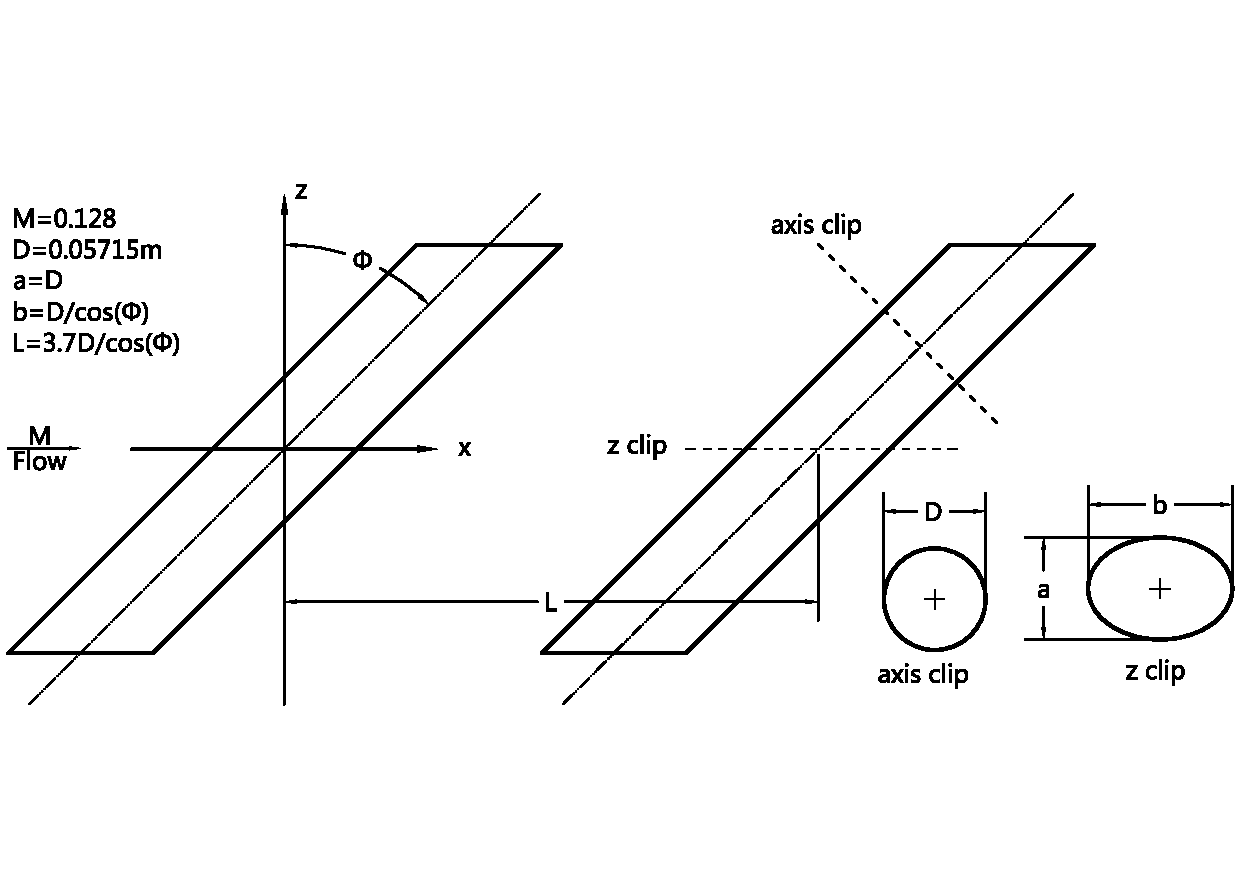
\includegraphics[width=12cm]{./img/Geom_pdf}
  \caption{插入一个pdf图片}
  \label{fig:visual}
\end{figure}

{\bf{实例3:}} 双列插入位图和矢量图:双列的实现依靠\textbackslash begin\{subfigmatrix\}\{2\}和\textbackslash end\{subfigmatrix\},插入图片命令为\textbackslash subfigure。

图片引用是分为单个图片引用和一起引用,例如引用自图片时~\ref{fig:subfig:Curve_jpg},引用全图时~\ref{fig:twoColns}。

\begin{figure}[htb]
\centering
 \begin{subfigmatrix}{2}                 % number of columns
  \subfigure[jpg位图格式]{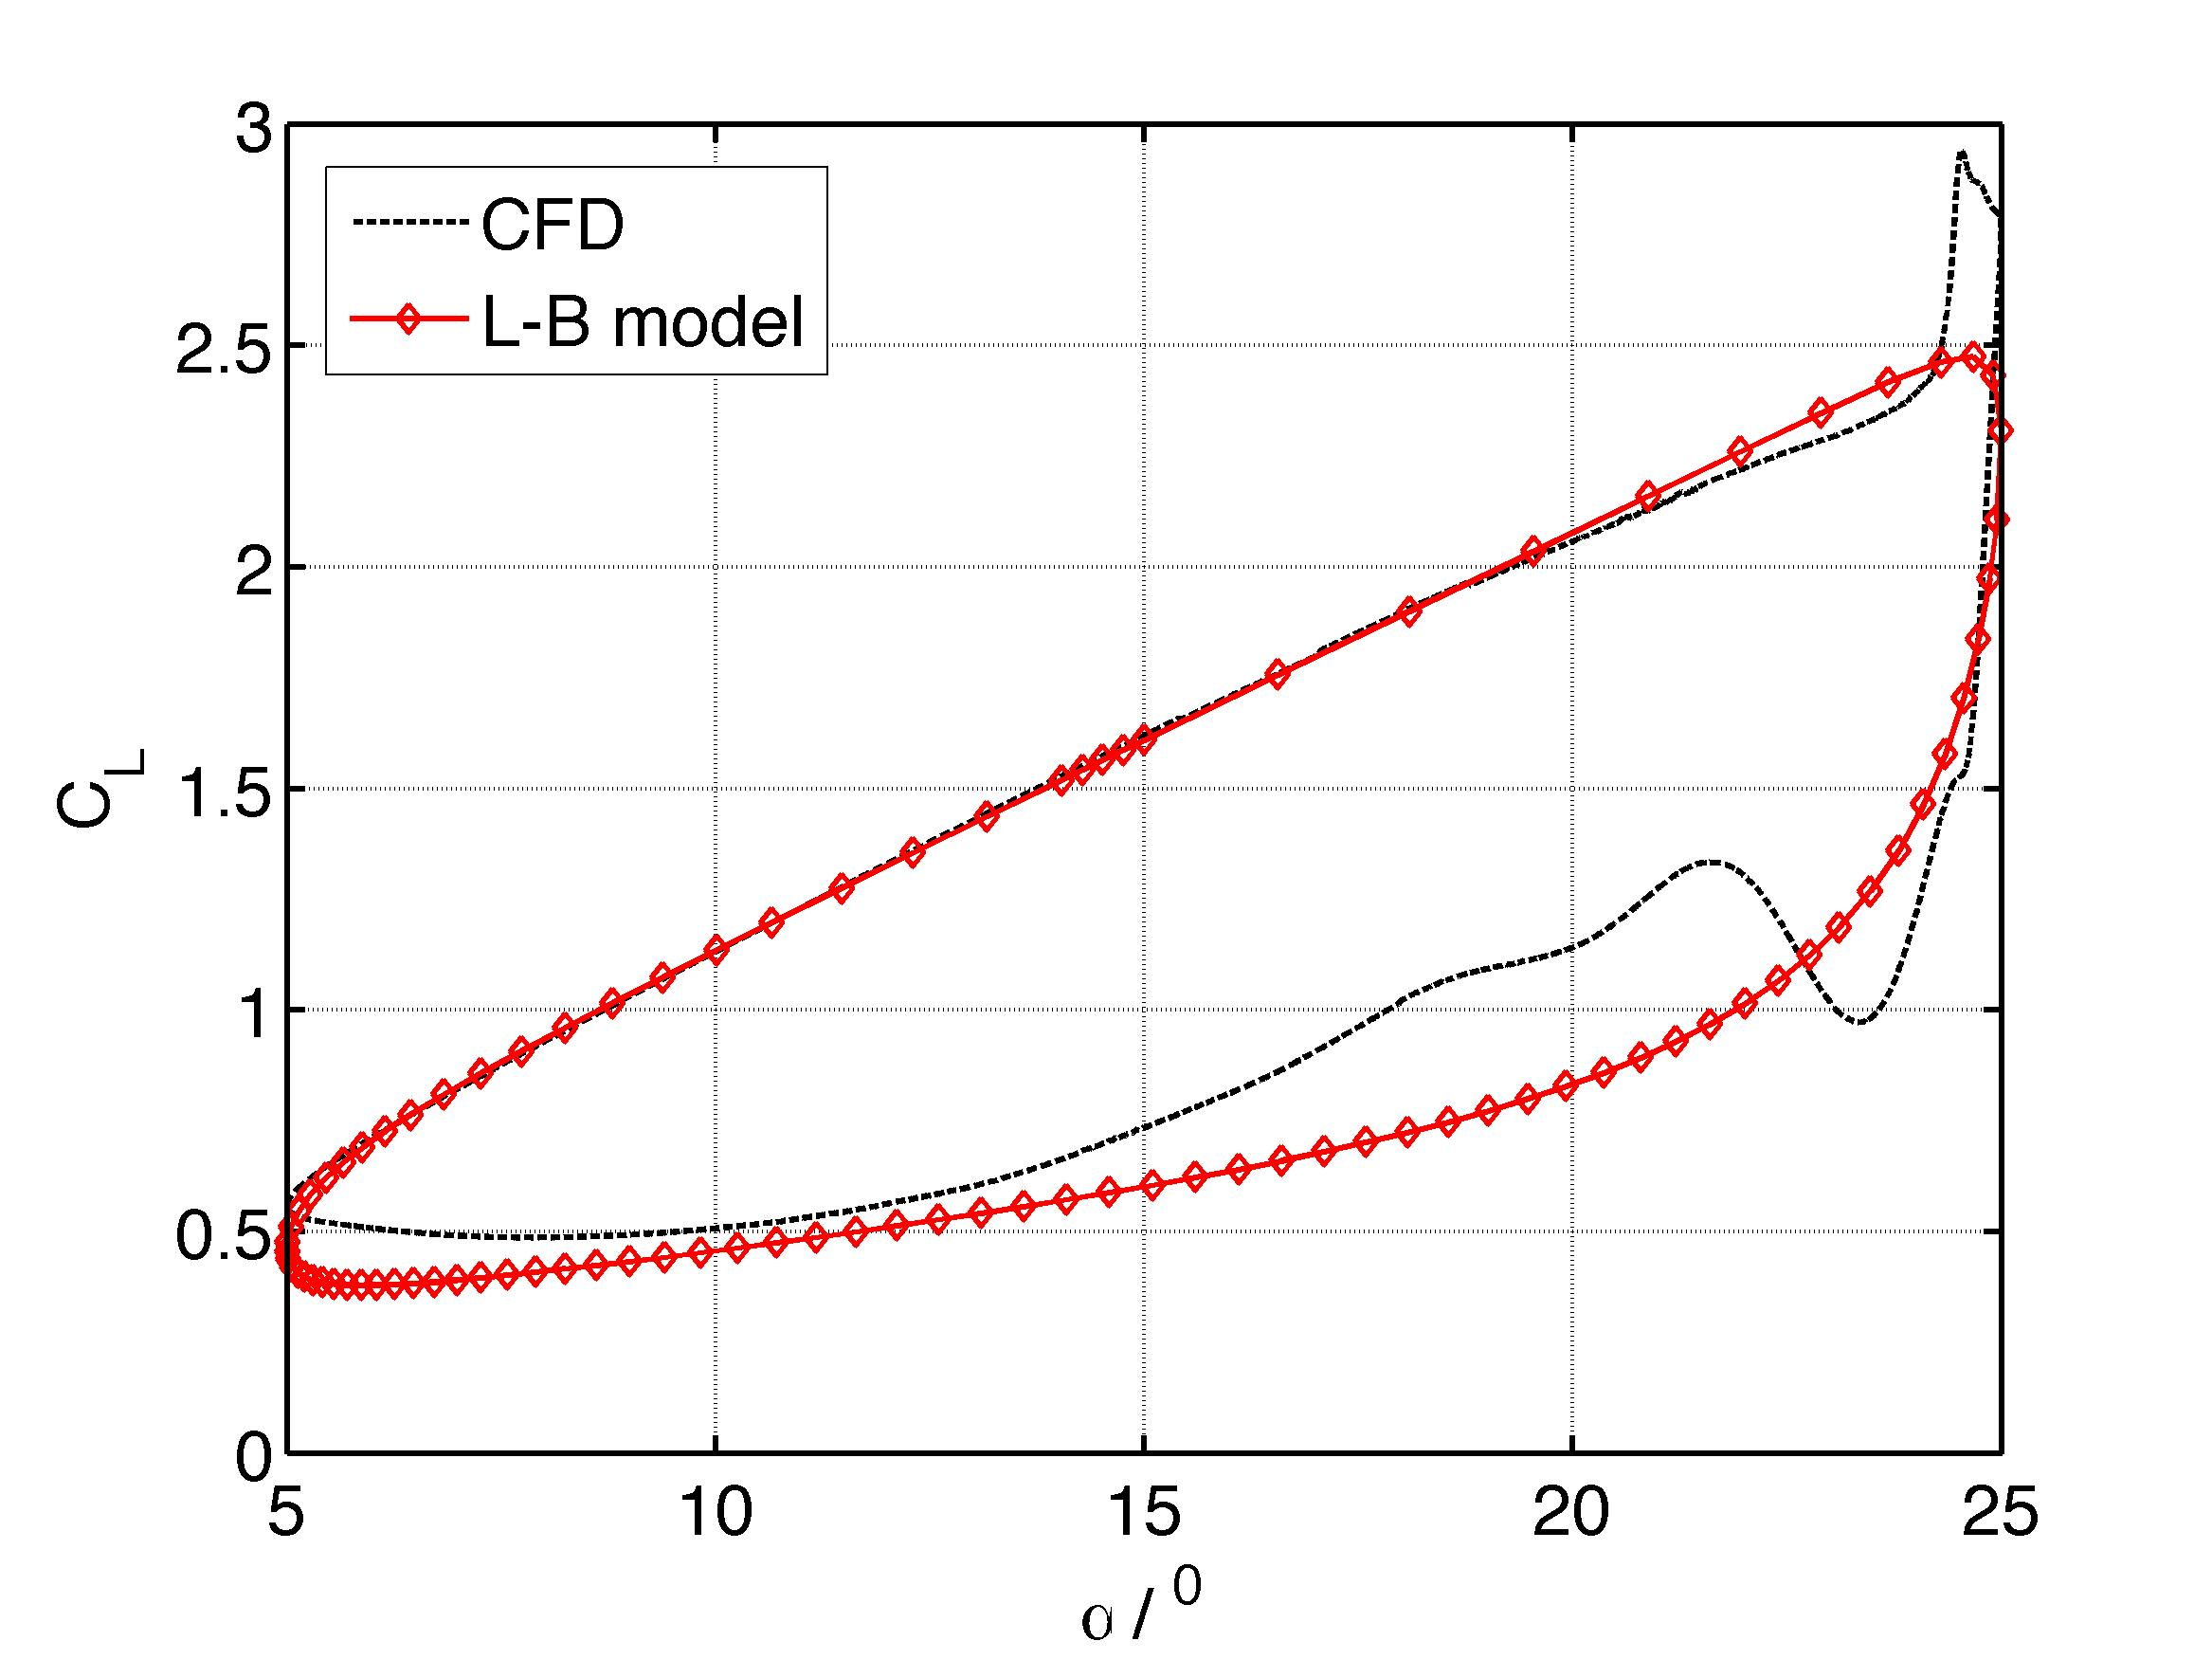
\includegraphics[width=6.5cm]{./img/Curve_jpg}
  \label{fig:subfig:Curve_jpg}}
  \subfigure[eps矢量图格式]{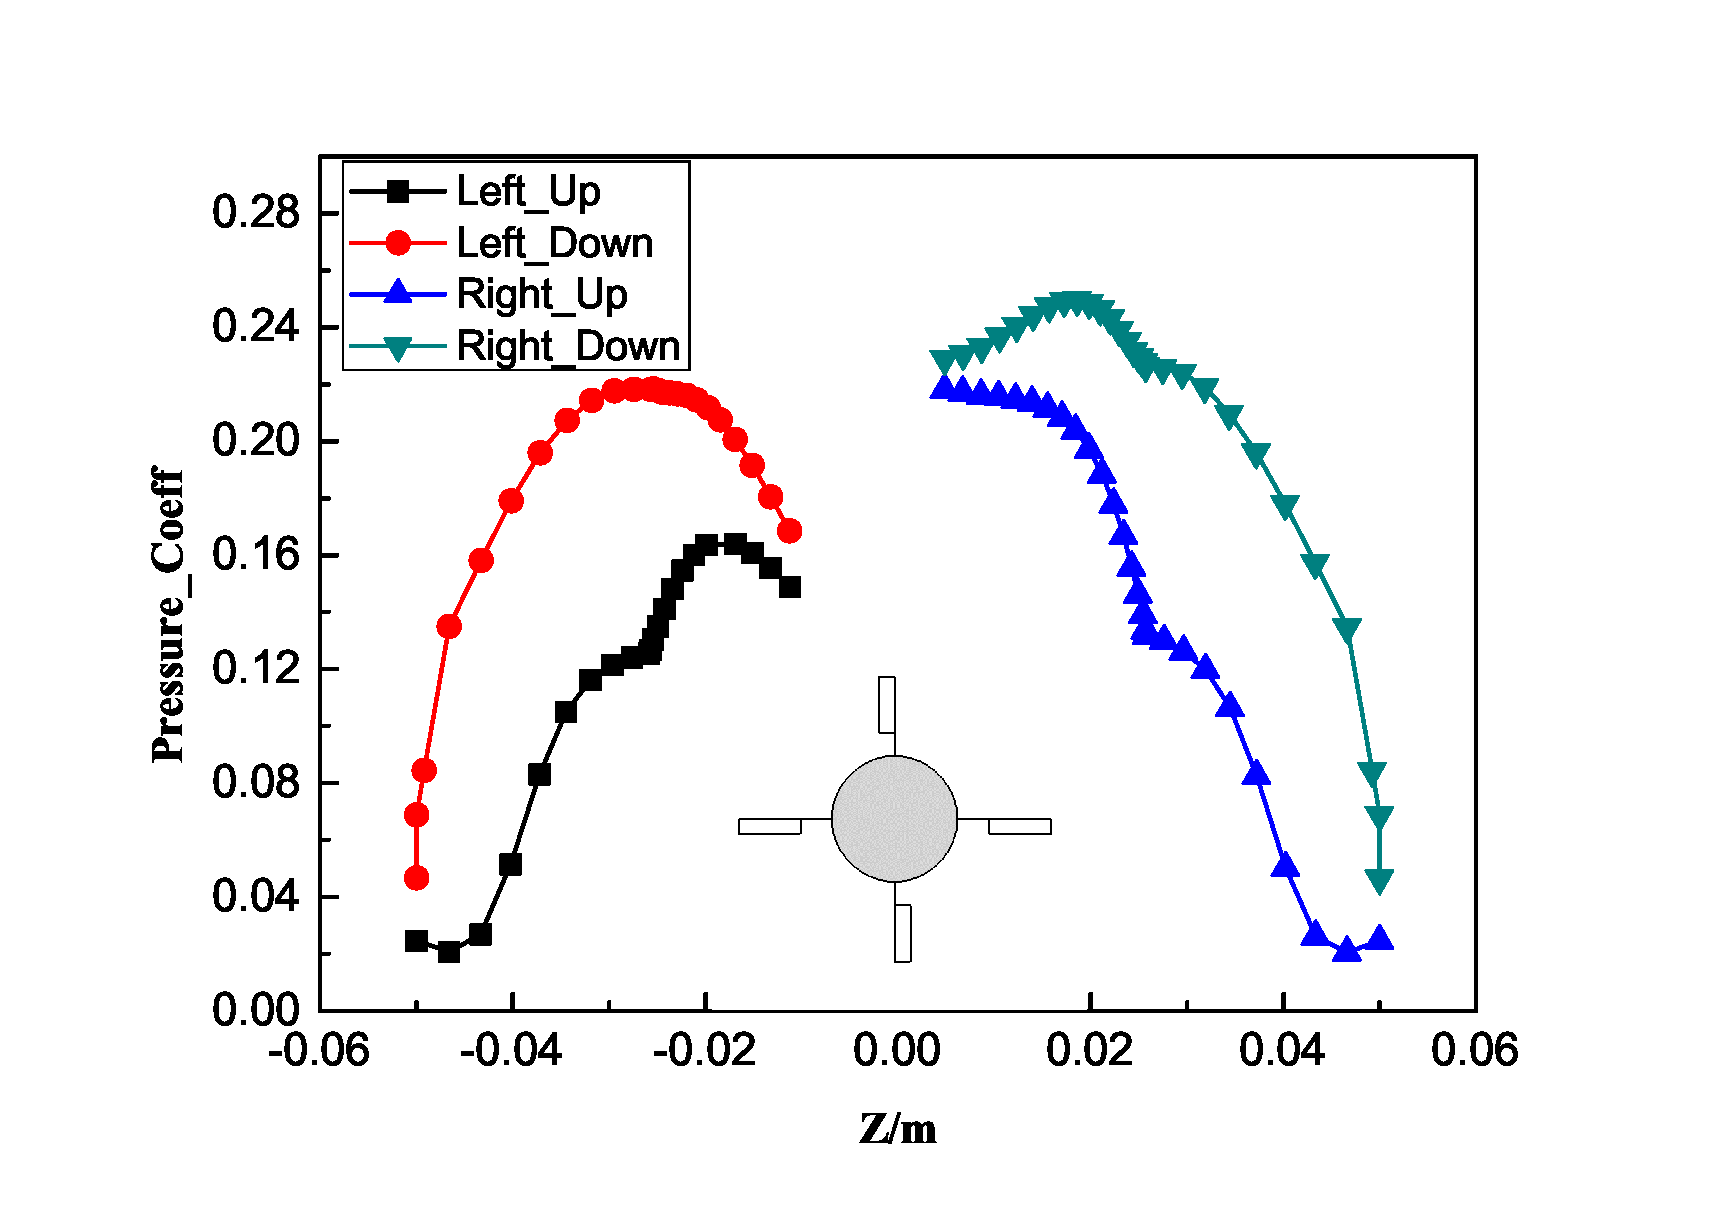
\includegraphics[width=7.5cm]{./img/plot_eps.eps}
  \label{fig:subfig:plot_eps}}
 \end{subfigmatrix}
 \caption{插入横排两列图片:a) jpg位图格式;b) eps矢量图格式}
 \label{fig:twoColns}
\end{figure}

{\bf{实例4:}} 单行两个图片插入:与实例3不同之处是这里是两个独立的图片,采用{\it\bf{minipage}}方式实现,引用是都是独立的进行引用,如图~\ref{fig:minipage:Curve_jpg}。

\begin{figure}[htb]           
\centering
\begin{minipage}[t]{0.45\linewidth}
    \centering
    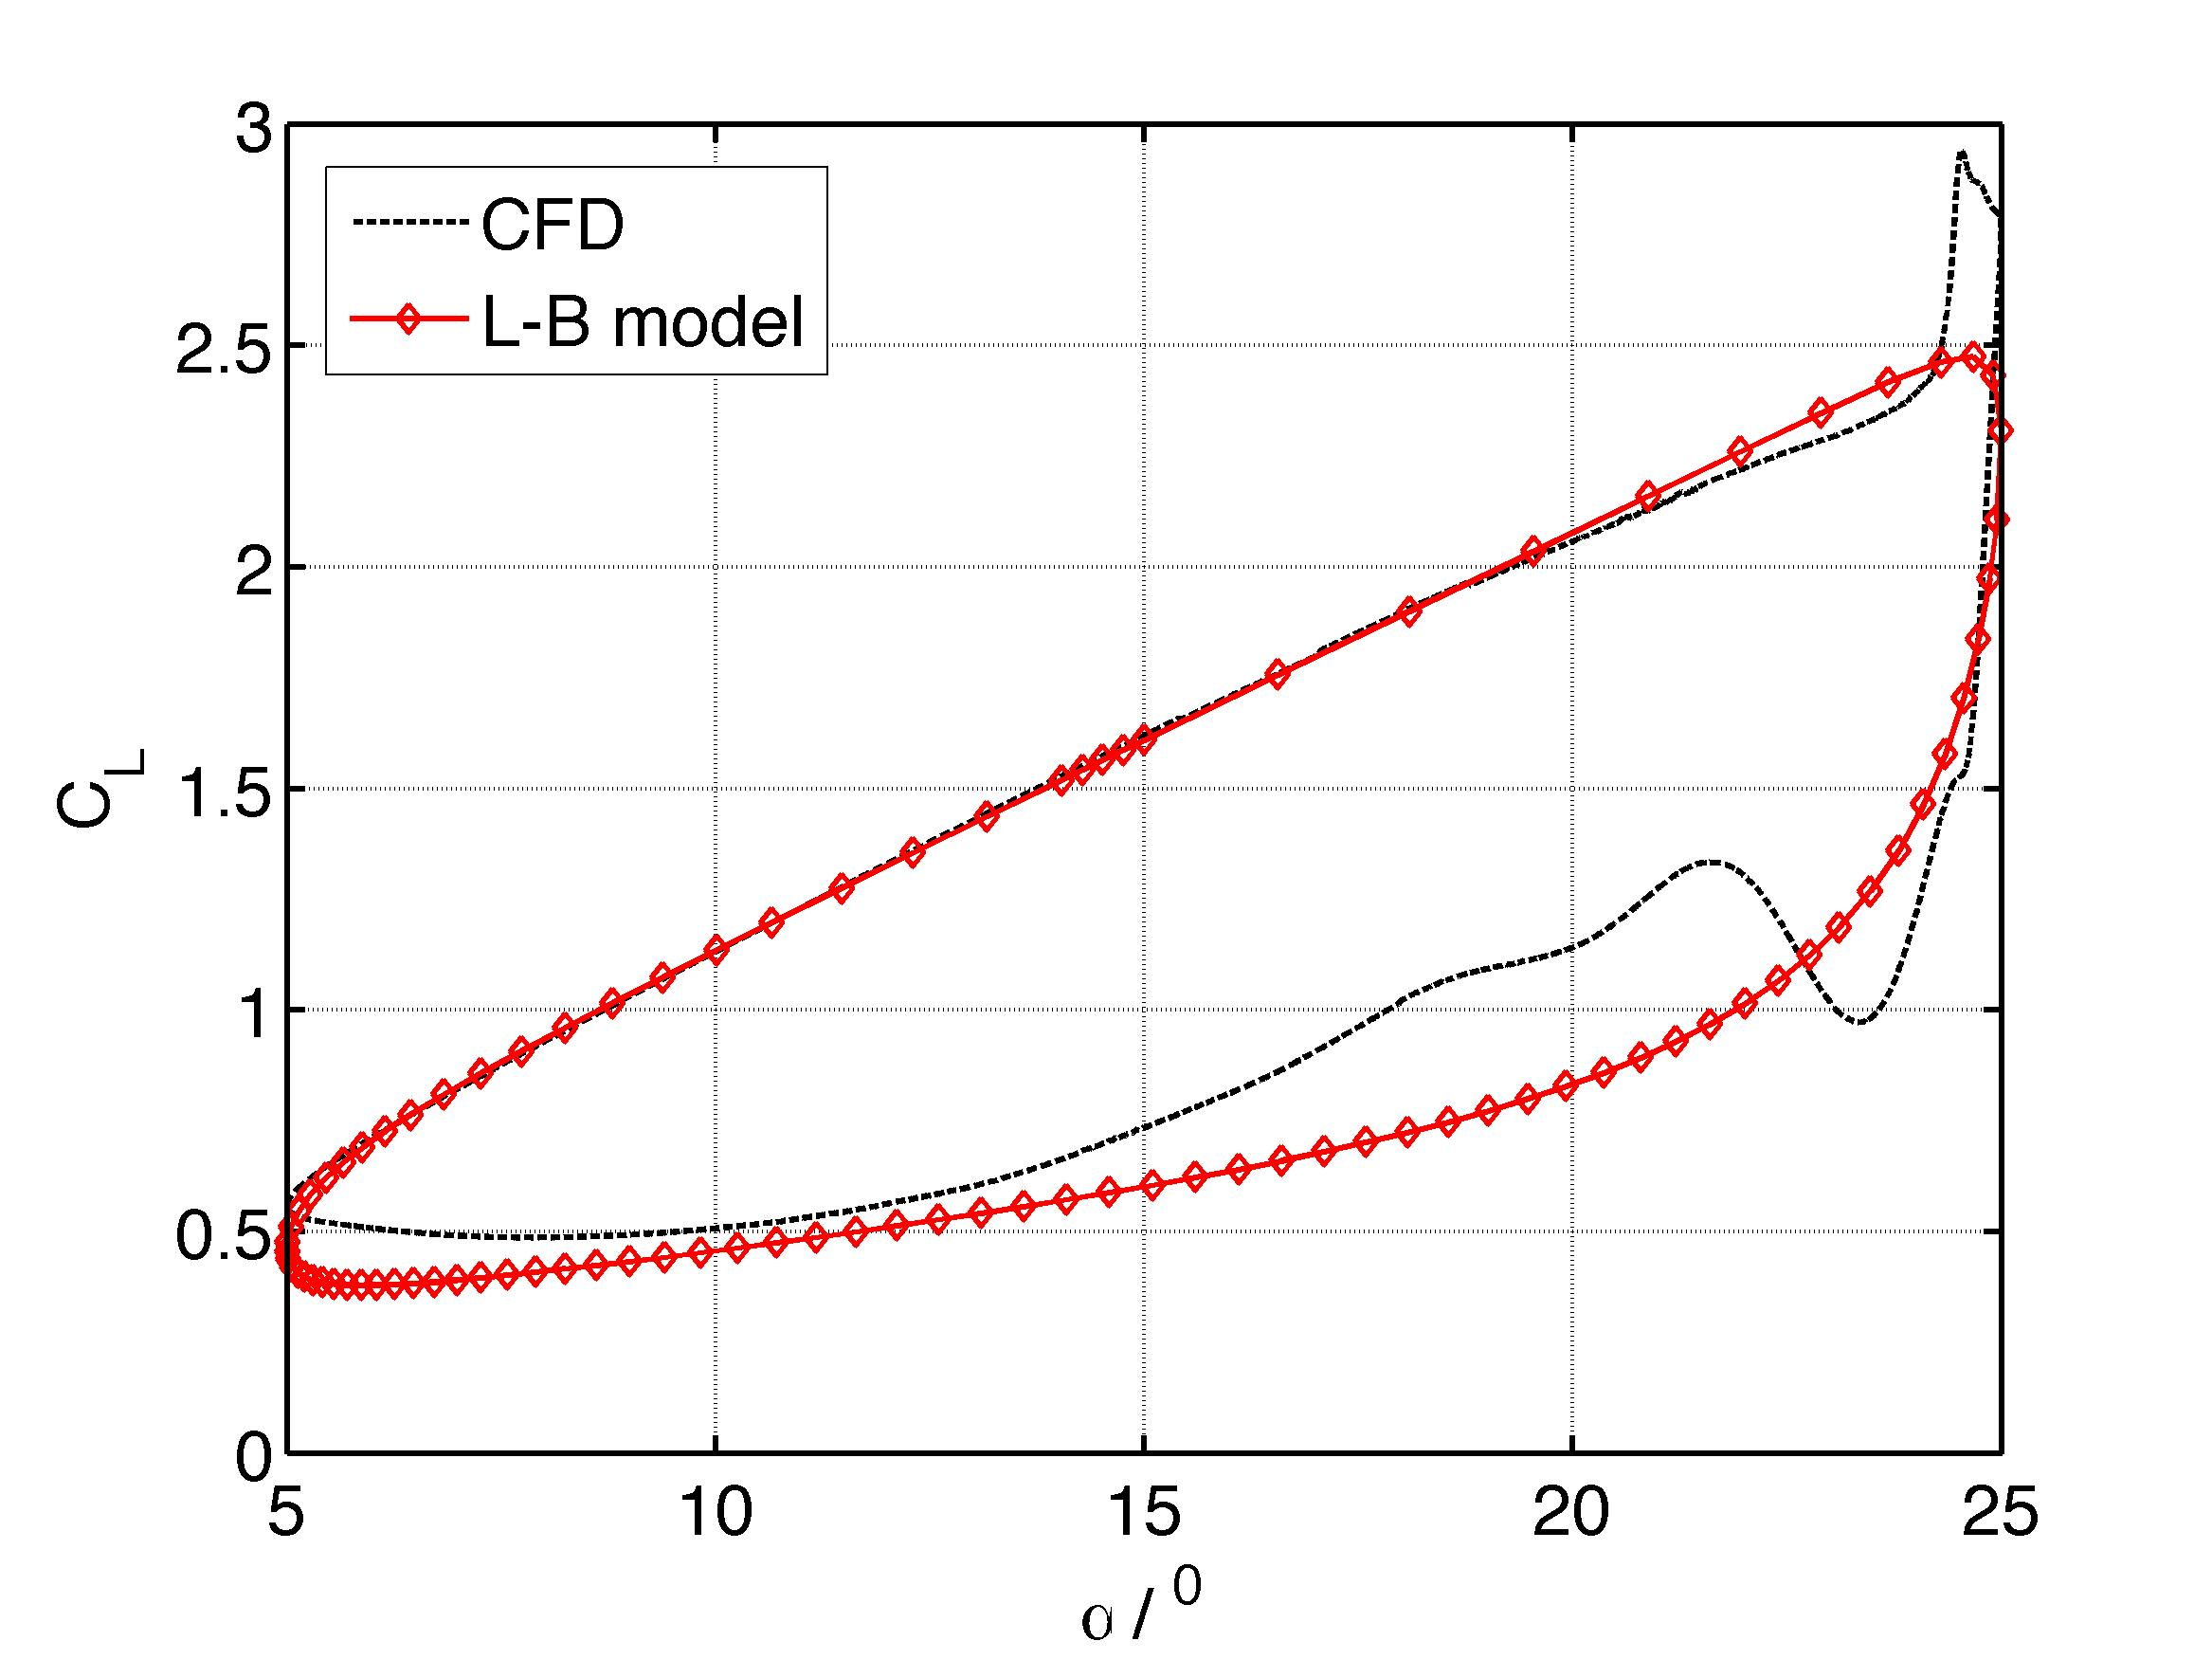
\includegraphics[width=6.5cm]{./img/Curve_jpg}
    \caption{jpg位图格式}
     \label{fig:minipage:Curve_jpg}
\end{minipage}
\hspace{3ex}                                             
\begin{minipage}[t]{0.45\linewidth}
    \centering
    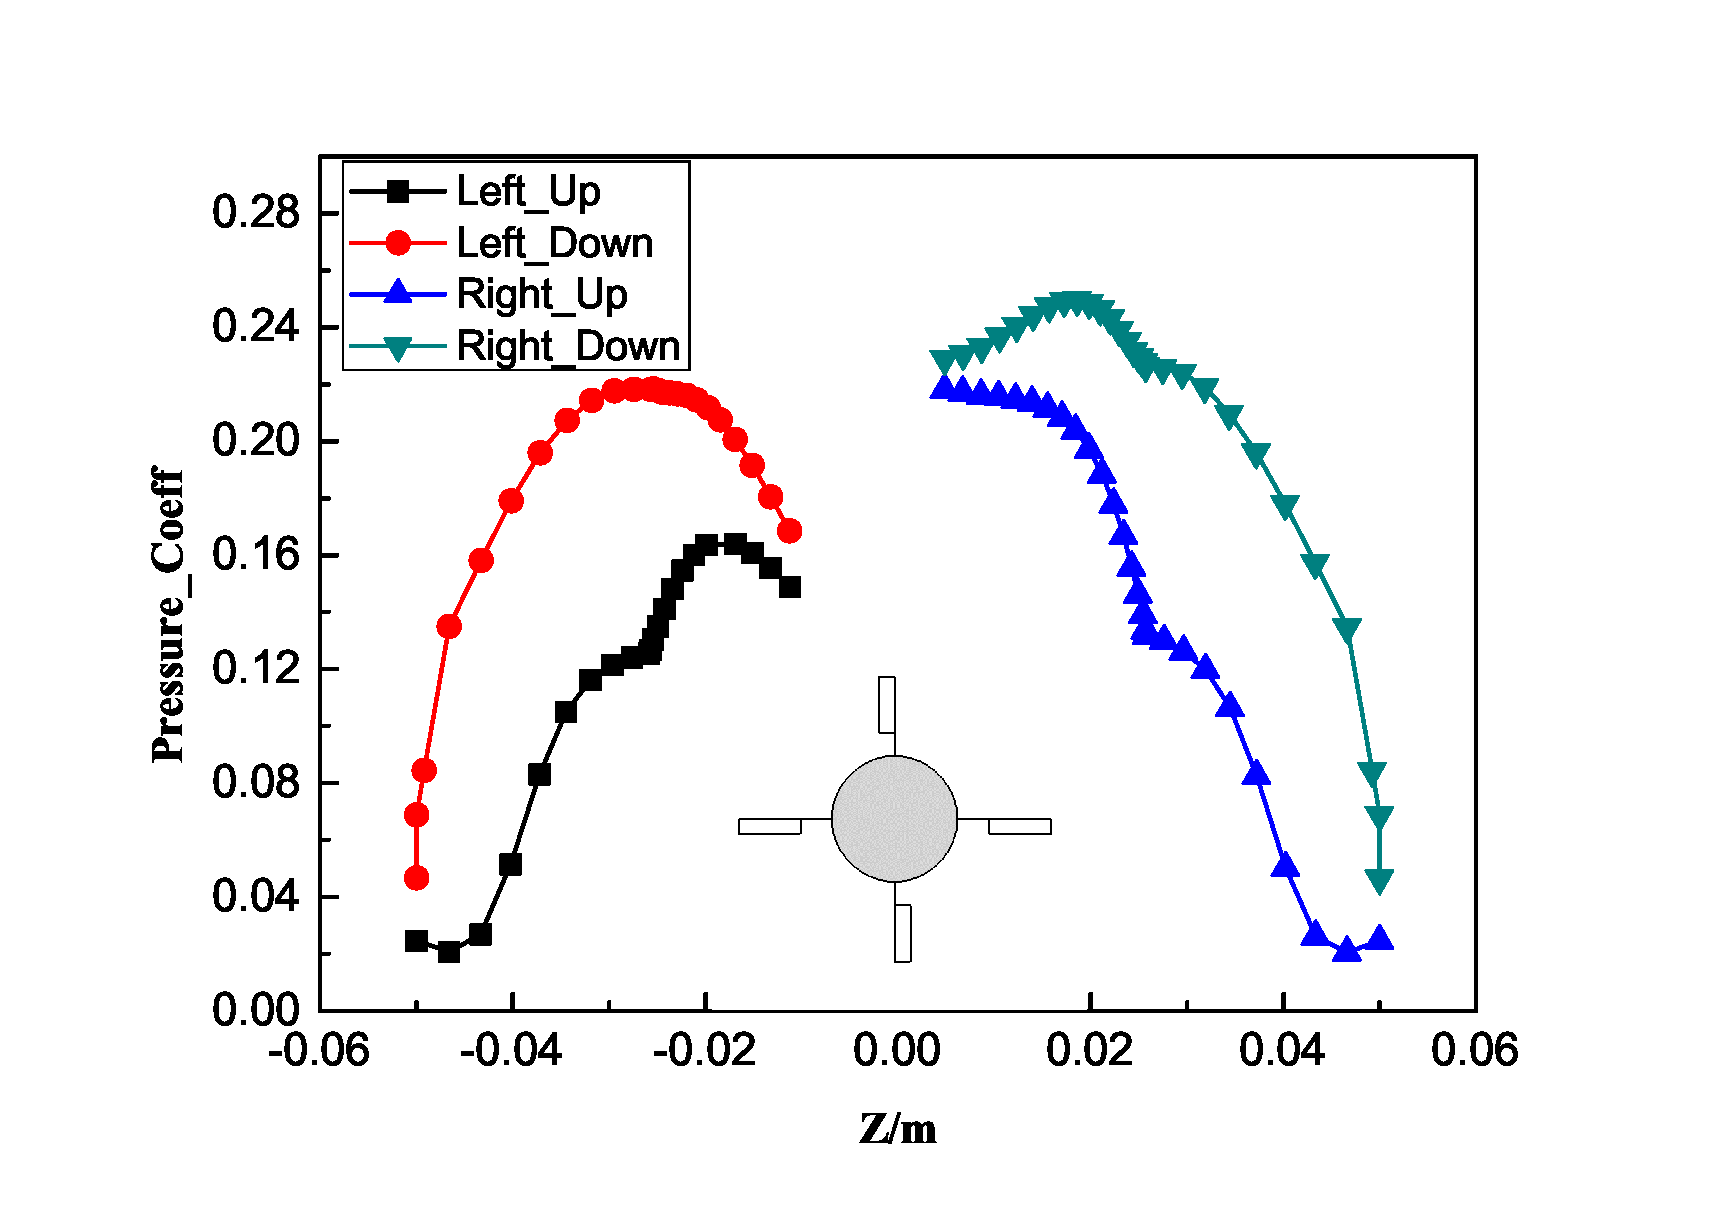
\includegraphics[width=7.5cm]{./img/plot_eps.eps}
    \caption{eps矢量图格式}
    \label{fig:minipage:plot_eps}
\end{minipage}
\end{figure}

{\bf{实例5:}} overpic在图片上进行文字标注:某些时候需要在图片上添加文字说明,并保持原图片格式,这里采用overpic的方法在图片上直接添加文字。

\begin{figure}[htb]
\centering
 \begin{overpic}[width=12cm]{./img/Geom_pdf}
   \put(-8,20){\rotatebox{90}{\footnotesize{纵坐标($r/s$)}}}
   \put(40,2){\footnotesize{手动添加横坐标 ($s$)}}
  \end{overpic}
\caption{在图片上添加文字说明}
\label{fig:overpic}
\end{figure}

尽管可以使用jpg、pdf、eps多种格式的图片,但是这里推荐优先使用eps或pdf的矢量图,提高图片的分辨率。在图片上添加文字说明优先使用overpic的方式,保留原图片。
%
%%%%% ------------------------------------------------------------------------------------------
%%
%%%%*********************************Appendix********************************************
%%
%% Some subordinate chapters.
\chapter{南京理工大学博士、硕士学位论文撰写格式}
\label{app:format}
为了规范博士、硕士学位论文的撰写,根据由国家标准局批准颁发的GB7713-87《科学技术报告、学位论文和学术论文的编写格式》,将博士、硕士学位论文的编写格式及有关标准统一规定如下:

详细参见研究生网站(http://gs.njust.edu.cn/a/xwgl/xwsq/20130508/82.html)。

\section{学位论文的装订}

博士、硕士学位论文页面设置一律为:上空30mm,下空24mm,左空25mm,右空25mm,对称页边距,页眉20mm,页脚20mm。用A4(297mm×210mm)标准大小的白纸,装订成册后尺寸为(292mm×207mm)。硕士论文封面用157g白色铜版纸,博士论文封面用230g黄色云彩纸。
封二、英文封二、声明和学位论文使用声明采用单页印刷,从中文摘要开始采用双面印刷。
正文中的一级标题(章目)用小3号加粗宋体,段前段后各空18磅,居左;二级标题(条)用4号加粗宋体,段前段后各空12磅,居左;三级标题(款)用小4号加粗宋体,段前段后各空6磅,居左;四级标题(项)同正文用小4号宋体,行距20磅。数字和字母采用Times New Roman体。样本详见附件。

学位论文格式为:( 注:页眉字体为小5号宋体)

奇数页眉:

博士/硕士论文\hspace{40pt}论文题目

偶数页眉:

章节号和名\hspace{40pt}/硕士论文


\section{学位论文前置部分}
\subsection{封面}
封面按统一的博士、硕士学位论文封面的内容和格式填写。(见附件一,注:密级部分如:秘密、机密或绝密必须填,其余可不填。密级后面★作标志,★后注明保密期限。)

书脊要注明学位论文题名及学位授予单位名称。

\subsection{封二}
学位论文的封二可作为封面标识项目的延续,内容包括学位论文级别、题目、作者、指导教师、作者单位、出版时间等。该页置于封面下面,包括中英文版,中文在前,英文在后。字体和字号以封面为准。见附件三和附件四。

\subsection{声明}
另页起,用附件五,对其内容不得作任何改动。该声明置于封二之后,中文摘要之前。

\subsection{摘要}
摘要是学位论文内容的不加注释和评论的简短陈述,说明研究工作的目的、实验方法、实验结果和最终结论等。应是一篇完整的短文,可以独立使用和引用,摘要中一般不用图表、化学结构式和非公知公用的符号和术语。标题用3号宋体加粗,居中,正文用小4号宋体。

摘要分中、外两篇,硕士论文摘要中文字数400~600个字,博士论文摘要中文字数800~1000个字。英文摘要的内容与中文摘要一致,且需合符语法,语句通顺。

摘要的装订按中、外文顺序进行,置于声明之后,分别由另页开始。详见附件六、七。

\subsection{关键词}
关键词是为了便于文献标引从该学位论文中选取出来用以表示全文主题内容信息款目的单词或术语,一般选取3~8个。其中关键词三个字用四号宋体加粗,其余用小4号宋体。

关键词写法的例:关键词:专家系统,模糊数学,枪械设计,知识库

关键词分为中、外文分别附在中、外文摘要的末尾。见附件六、七。

\subsection{目次页}
目次页由学位论文的一、二、三级标题、致谢、参考文献、附录等的序号、名称和页码组成,目次页置于外文摘要后,由另页开始。其中目录两字用3号宋体加粗,一级标题、致谢、参考文献、附录等用4号加粗宋体,其余为小4号宋体。见附件八。

\subsection{图表清单}
如遇图表较多,可以分别列出清单,清单置于目次页后,由另页开始。本条为非必要部分。图的清单应有序号、图名和页码。表的清单应有序号、表名和页码。图表清单置于目次页之后,由另页开始。“图表目录”四字用3号宋体加粗,其余用小4号宋体。正文中表说用5号宋体在表上,图说用5号宋体在图下,图表内的字体用5号宋体。如论文中无图表,此项可免。见附件九。

\subsection{注释表}
注释表为符号、标志、缩略词、首字母缩写、计量单位、名词和术语等的注释说明汇集表,置于图表清单后,由另页开始,本条为非必要部分。

\subsection{注释}
当论文中的字、词或短语需要进一步加以说明或标明具体的文献来源时,用注释。注释采取集中著录在“文后”或分散著录在“脚注”。

论文“文后”集中注释示例:

①国家自然科学基金项目(30070218)。

②傅深渊(1963-),男,浙江省××人,毕业于××大学××专业,……。 

…………。

论文“脚注”分散著录注释示例:

①国家自然科学基金项目(30070218)。

②傅深渊(1963-),男,浙江省××人,毕业于××大学××专业,……。

…………。

\section{学位论文的主要部分}
详见附件十、十一、十二、十三。

\subsection{引言(或绪论)}
引言(或绪论)简要说明研究工作的目的、范围、前人的工作和知识空白、理论基础和分析、研究设想、研究方法、实验设计、预期结果和意义等。引言(或绪论)不要与摘要雷同,一般教科书有的知识,在引言中不必赘述。

引言(或绪论)重点应放在有关历史回顾和前人工作的综合评述,以及理论分析等,应该用足够的文字叙述,如有必要可单独编成第一章。详见附件十。

\subsection{正文}
正文是学位论文的核心部分,要求做到客观真切,准确完备,合乎逻辑,层次分明,简练可读。

正文按一级标题(章)、二级标题(条)、三级标题(款)、四级标题(项)的次序编排,其中的图表等的序号归入本身所处的本层次的次序中(见图3.2.1)

\subsubsection{图}
图应有图名、图号及必要的说明。

图应具有“自明性”,即只看图、图名和图例,不阅读正文,就可理解图意。必要时应将图上的符号、标记、代码或实验条件等用最简练的文字,横排于图名的下方。曲线图的纵横坐标应标注量纲及标准规定的符号,只有在不必要标明(如无量纲等)的情况下方可省略。

图号按章编排,图名在图号之后空一格排写,图中若有分图时用a)、b)等置于分图之下。如第四章第一个图的图号及图名:图4.1 和通关系证明示意图

%
%%%%% ------------------------------------------------------------------------------------------
%%
%%%%********************************Backmatter*******************************************
%%
%% Matters of Bibliography, Glossary, Index.
\backmatter
%%
%%% >>> Acknowledgements
%%
\begin{thanks}

值此论文完成之际,谨在此向多年来给予我关心和帮助的老师、学长、同学、
朋友和家人表示衷心的感谢!

没有~ctex package~的众多前辈的辛勤付出和~CASthesis和~NJUSTthesis-latex808作者的贡献,
~\LaTeX{}~菜鸟的我是无法完成此学位论文模板的。在~\LaTeX{}~中的一点一滴的成长源于
开源社区的众多资料和教程,在此对所有前辈们的付出表示感谢!

在这里感谢下载该模版并在使用中提出宝贵意见的朋友们!特别的,笔者在这里感谢\texttt{veemy}在中文CTeX上提出的问题探讨,问题解决了在texlive-2015上的应用问题,链接如下:

\url{http://bbs.ctex.org/forum.php?mod=viewthread&tid=151973&extra=&page=1}

其中,在交流过程中得到了CTeX版主\texttt{LiamHuang}(\url{http://liam0205.me/about/})的指导,特别感谢!

......

\vskip 18pt

谨把本文献给我最敬爱的父亲!

\end{thanks}
%%
%%% >>> Bibliography
%%
%\bibliographystyle{plainnat}
{\centering\bibliography{bib/myRefs}}%
%%
%%% >>> Publications
%%
\begin{publications}{99}
\item[] {\bf{攻读博士学位期间发表的论文和出版著作情况:}}

\item Thesis Template of the Nanjing University of Science \& Technology, GitHub$^{\circledR}$, 2015.

\vspace{1.0cm}
\item[] {{\songti\zihao{4}\bf{攻读博士学位期间参加的科学研究情况:}}}
\setcounter{enumiv}{0}

\item \texttt{njustThesis}:南京理工大学论文\LaTeX{}模版,自拟兴趣课题,完成模版的代码和说明文档的编写.


\end{publications}

%%
%%% >>> Resume
%%

\begin{resume}

\begin{resumesection}{njustThesis~作者基本情况}
程杰,男,安徽霍山人,1989年出生,南京理工大学机械工程学院博士研究生。
\end{resumesection}

\begin{resumelist}{联系方式}
通讯地址:江苏省南京市玄武区孝陵卫200号,南京理工大学机械工程学院202教研室

邮编:210094

E-mail: jie.cheng@aliyun.com
\end{resumelist}

\end{resume}

%%
\end{document}
%%%%% ------------------------------------------------------------------------------------------
